\documentclass[a4paper]{article}

\usepackage{INTERSPEECH2015}

\usepackage{graphicx}
\usepackage{amssymb,amsmath,bm}
\usepackage{textcomp}

\def\vec#1{\ensuremath{\bm{{#1}}}}
\def\mat#1{\vec{#1}}

\usepackage{cleveref}
\usepackage{caption}

\usepackage[dvipsnames]{xcolor}
\newcommand{\TODO}[1]{{\color{red}\textbf{[TODO #1]}}}

\sloppy % better line breaks
\ninept

\title{A CAPT tool for training and research on lexical stress errors in German}

%%%%%%%%%%%%%%%%%%%%%%%%%%%%%%%%%%%%%%%%%%%%%%%%%%%%%%%%%%%%%%%%%%%%%%%%%%
%% If multiple authors, uncomment and edit the lines shown below.       %%
%% Note that each line must be emphasized {\em } by itself.             %%
%% (by Stephen Martucci, author of spconf.sty).                         %%
%%%%%%%%%%%%%%%%%%%%%%%%%%%%%%%%%%%%%%%%%%%%%%%%%%%%%%%%%%%%%%%%%%%%%%%%%%
%\makeatletter
%\def\name#1{\gdef\@name{#1\\}}
%\makeatother
%\name{{\em Firstname1 Lastname1, Firstname2 Lastname2, Firstname3 Lastname3,}\\
%      {\em Firstname4 Lastname4, Firstname5 Lastname5, Firstname6 Lastname6,
%      Firstname7 Lastname7}}
%%%%%%%%%%%%%%% End of required multiple authors changes %%%%%%%%%%%%%%%%%

\makeatletter
\def\name#1{\gdef\@name{#1\\}}
\makeatother \name{{\em%
  Anjana Sofia Vakil
  %Author Name$^1$, Co-author Name$^2$
  }}

\address{%
  %$^1$Author Affiliation \\
  %$^2$Co-author Affiliation \\
  Department of Computational Linguistics \& Phonetics\\
  Saarland University, Saarbr\"{u}cken, Germany\\
  {\small \tt 
  anjanav@coli.uni-saarland.de}
}
%\twoauthors{Karen Sp\"{a}rck Jones.}{Department of Speech and Hearing \\
%  Brittania University, Ambridge, Voiceland \\
%  {\small \tt Karen@sh.brittania.edu} }
%  {Rose Tyler}{Department of Linguistics \\
%  University of Speechcity, Speechland \\
%  {\small \tt RTyler@ling.speech.edu} }

%
\begin{document}

  \maketitle
  %
  \begin{abstract}
    %This demonstration presents a prototype tool for Computer-Assisted Pronunciation Training (CAPT) in German.  
    This demonstration presents \textbf{de-stress}: the German (\textbf{de}) \textbf{S}ystem for \textbf{T}raining and \textbf{R}esearch on \textbf{E}rrors in \textbf{S}econd-language \textbf{S}tress \cite{destress}. 
    This prototype Computer-Assisted Pronunciation Training (CAPT) tool provides a variety of options for diagnosis of and feedback on lexical stress errors, and could potentially be a useful component of an intelligent CAPT system.
  \end{abstract}
  \noindent{\bf Index Terms}: CAPT, German, prosody


	%\section{System overview}
	
%	This demonstration presents \textbf{de-stress}\footnote{\texttt{github.com/vakila/de-stress}}: the German (\textbf{de}) \textbf{S}ystem for \textbf{T}raining and \textbf{R}esearch on \textbf{E}rrors in \textbf{S}econd-language \textbf{S}tress. 
%%
%%Implemented as a web application 
%%%in the Java-based language Groovy\footnote{\texttt{groovy-lang.org}} using the Grails web framework,\footnote{\texttt{grails.org}} 
%%de-stress and its source code are openly available online.\footnote{\texttt{github.com/vakila/de-stress}}
%%
%%\Cref{fig:hourglass-ITS} provides a conceptual overview of the tool, which 
%This prototype CAPT tool provides a variety of options for diagnosis of and feedback on lexical stress errors, and could potentially be a useful component of an intelligent CAPT system. 
%

\section{A training tool for German learners}

 Via a simple web interface, de-stress presents a learner with a German sentence,
 %(taken from the IFCASL corpus), 
 with one of the words highlighted as the target word for that exercise. The learner is prompted to submit an utterance of that sentence for assessment and feedback, with the instruction to focus on the accurate expression of the lexical stress pattern of the target word. The prosody (duration, fundamental frequency, and intensity) of the learner's utterance is then analyzed using the speech processing software JSnoori \cite{jsnoori}. Based on this analysis, lexical stress errors are diagnosed via either classification-based error detection using machine learning \cite{Vakil2015}, or comparison of the learner's utterance with one or more reference utterances by native speakers. In the comparative approach, references may be selected manually, or by automatically selecting the closest match(es) to the learner's voice (fundamental frequency). 
 
 Based on this error diagnosis, the learner is presented with one or more types of feedback on their realization of lexical stress, with options including visual feedback via abstract graphical visualizations and/or text stylization (see \cref{fig:interface:student}), auditory feedback via prosodic modification of the learner's utterance, verbal error/success messages, and graphical ``skill bars'' corresponding to each of the prosodic parameters analyzed.  Learners may also be asked to self-assess their utterance before viewing the system's diagnosis and feedback.
 %\Cref{fig:interface:student} presents a screenshot of the interface presenting such feedback.
% Unlike with some existing CAPT tools which rely on more direct signal visualizations (e.g. spectrograms, pitch contours) for feedback,
% %for diagnosis and feedback on pronunciation errors, 
% learners can interact with the tool and interpret its feedback independently, i.e. without the assistance of a human instructor at their side.




\section{A tool for teachers and researchers}
In addition to the learner-facing interface, 
%the tool also implements an interface through which 
the administrative interface of de-stress allows
language teachers or researchers of L2 language acquisition 
%can 
to
create new exercises for learners to complete, where each exercise features a specific combination of the various diagnostic methods and feedback types available in the system (see \cref{fig:interface:admin}).
By allowing fine-grained control over these features, de-stress allows teachers to create exercises matching the specific needs of their students, and enables researchers to study the 
%effectiveness of 
impact of
different diagnosis/feedback configurations
 %
%The 
%%teacher- or researcher-facing
%administrative interface for exercise creation can be seen in \cref{fig:interface:teacher}.
%
%	\begin{figure}[htbp]
%		\centering
%		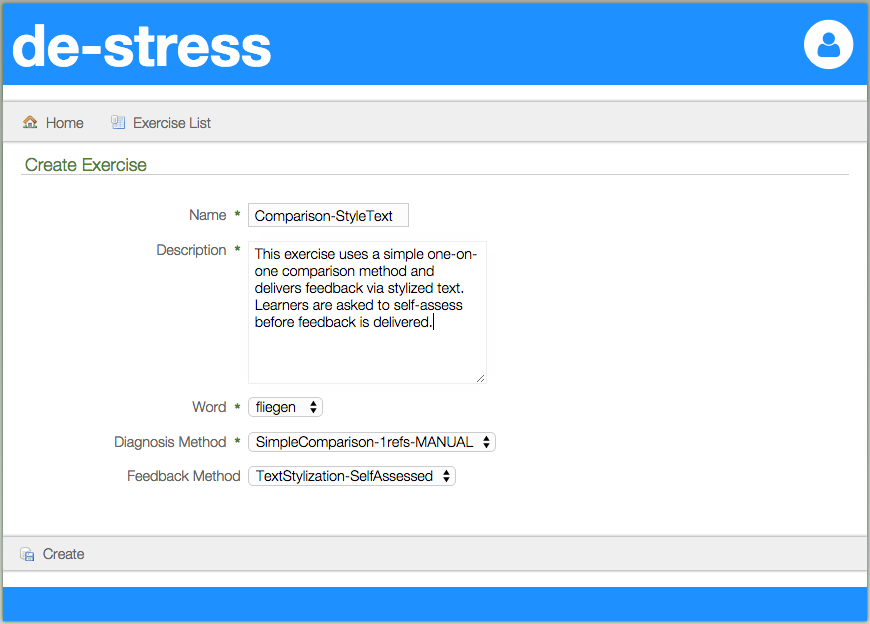
\includegraphics[width=\columnwidth]{../../img/screenshots/TeacherInterface-userIcon}
%		\caption{The interface of de-stress for teachers/researchers}
%		\label{fig:interface:teacher}
%	\end{figure}
%
%\TODO{This prototype tool} has thus been developed with both instructional and research applications in mind.
%Both instructional and research applications have thus motivated the development of de-stress.
%
%At the same time, researchers can use this modular system to study the impact of various assessment and feedback types 
on learner outcomes, user engagement, and other factors impacting the success of a CAPT system. 
%
Once more is known about which diagnosis/feedback types
are most effective 
% should be delivered to which learners 
in which situations, this tool could become a useful component of an intelligent CAPT system, in which 
%learner models and other intelligent components
models of relevant aspects of the learning context (e.g. the learner's skill level, learning progress, or personal preferences)
are used to automatically choose the most appropriate diagnostic and feedback methods. %, as \cref{fig:hourglass-ITS} illustrates.


	\begin{figure}[h!]
		\centering
		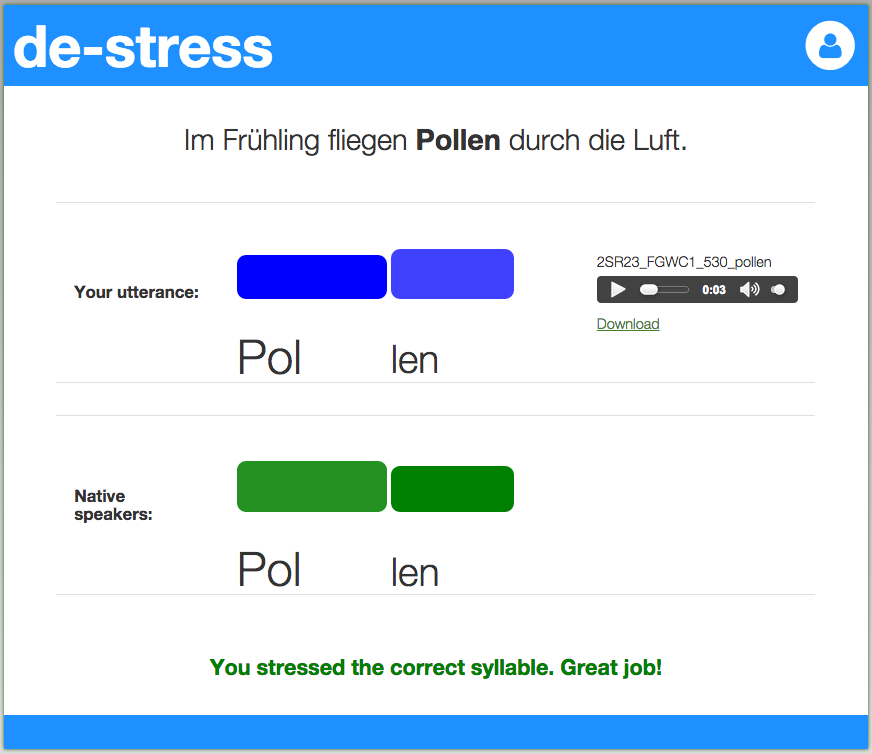
\includegraphics[height=5.7cm]{../../img/screenshots/StudentInterface-userIcon}
		\caption{Student-facing interface of de-stress, showing example of feedback delivery.}
%		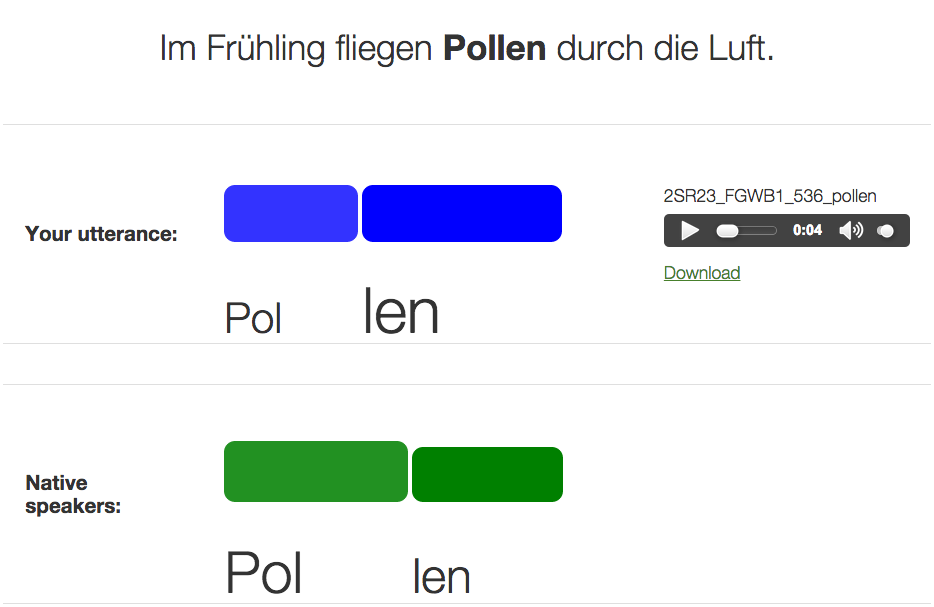
\includegraphics[width=\columnwidth]{../../img/screenshots/graphicalFB-weka-plusTextStyle}
%		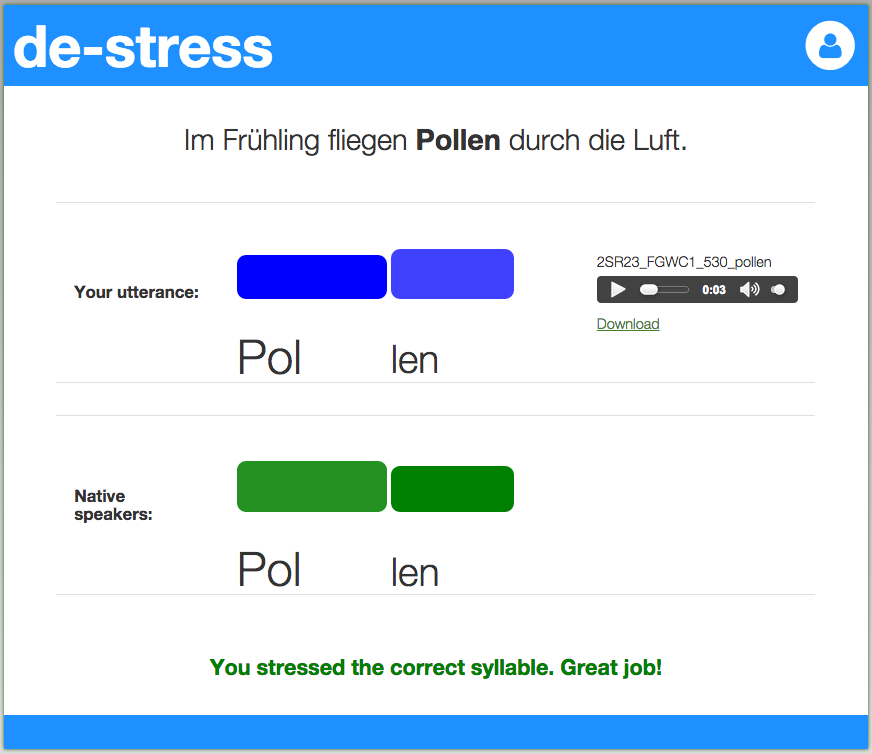
\includegraphics[width=\columnwidth]{../../img/screenshots/StudentInterface-userIcon}
%		\caption{Example of feedback delivery in de-stress}
		\label{fig:interface:student}
	\end{figure}
	
		\begin{figure}[h!]
		\centering
		\fcolorbox{gray!50}{white}{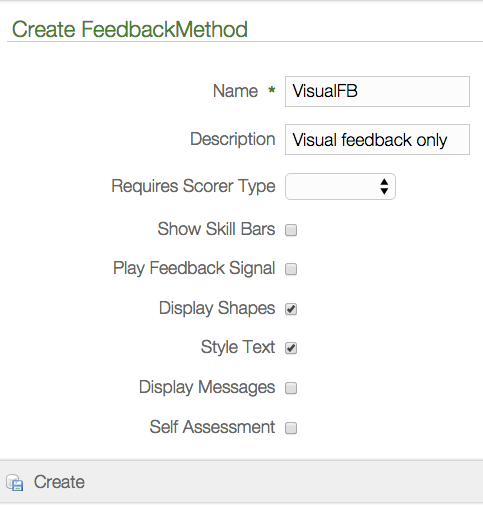
\includegraphics[height=5.4cm]{FeedbackMethod}}
		\caption{Administrative interface offering control over the feedback types delivered to the learner.}
		\label{fig:interface:admin}
	\end{figure}
	
%	\begin{figure}[!h] 
%		\centering
%		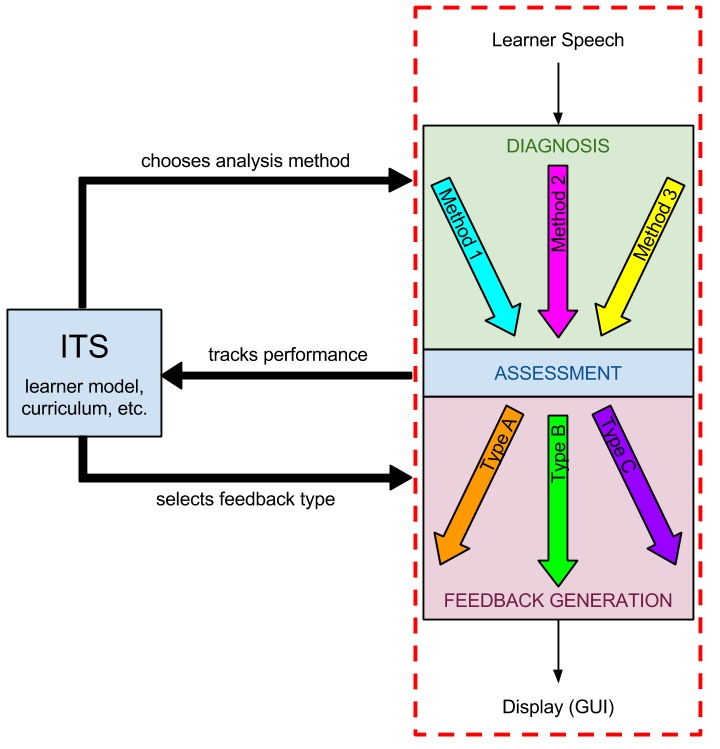
\includegraphics[height=.25\textheight]{../../img/hourglass-ITS} 
%		\caption[Conceptual diagram of the prototype lexical stress CAPT tool]{Conceptual diagram of the prototype 
%		%lexical stress CAPT 
%		tool 
%		(demarcated by dashed line) 
%		and its possible function in the context of an Intelligent CAPT System (ITS).}
%		\label{fig:hourglass-ITS}
%	\end{figure}
	
%	\section{Error diagnosis options}
%	\label{sec:diag}
%	
%	\TODO{}
%	
%	\section{Feedback options}
%	\label{sec:fb}
%	
%	\TODO{}
	
	


  %\newpage
  \eightpt
  \bibliographystyle{IEEEtran}

  \bibliography{demo}
  
%  \begin{thebibliography}{1}
%  \bibitem[1]{destress}
%  A.\ Vakil, de-stress [Online]. Available: github.com/vakila/de-stress
%  \bibitem[2]{jsnoori}
%  LORIA Speech Team, JSnoori [Online]. Available: jsnoori.loria.fr
%  \end{thebibliography}

%  \begin{thebibliography}{9}
%    \bibitem[1]{Davis80-COP}
%      S.\ B.\ Davis and P.\ Mermelstein,
%      ``Comparison of parametric representation for monosyllabic word recognition in continuously spoken sentences,''
%      \textit{IEEE Transactions on Acoustics, Speech and Signal Processing}, vol.~28, no.~4, pp.~357--366, 1980.
%    \bibitem[2]{Rabiner89-ATO}
%      L.\ R.\ Rabiner,
%      ``A tutorial on hidden Markov models and selected applications in speech recognition,''
%      \textit{Proceedings of the IEEE}, vol.~77, no.~2, pp.~257-286, 1989.
%    \bibitem[3]{Hastie09-TEO}
%      T.\ Hastie, R.\ Tibshirani, and J.\ Friedman,
%      \textit{The Elements of Statistical Learning -- Data Mining, Inference, and Prediction}.
%      New York: Springer, 2009.
%    \bibitem[4]{YourName15-XXX}
%      F.\ Lastname1, F.\ Lastname2, and F.\ Lastname3,
%      ``Title of your INTERSPEECH 2015 publication,''
%      in \textit{Interspeech 2015 -- 16\textsuperscript{th} Annual Conference of the International Speech Communication Association, September 06--10, Dresden, Germany, Proceedings}, 2015, pp.~100--104.
%  \end{thebibliography}

\end{document}
